% -*- coding: utf-8 -*-
%-------------------------designed by zcf--------------
\documentclass[UTF8,a4paper,10pt]{ctexart}
\usepackage[left=3.17cm, right=3.17cm, top=2.74cm, bottom=2.74cm]{geometry}
\usepackage{amsmath}
\usepackage{graphicx}
\usepackage{float}
\usepackage{cite}
\usepackage{caption}
\usepackage{enumerate}
\usepackage{booktabs} %表格
\usepackage{multirow}
\usepackage{enumitem}
\usepackage{subcaption}
\usepackage{tikz}%用于绘制流程图
\usepackage{float} % 如果需要 [H]
\usetikzlibrary{positioning}
\usetikzlibrary{shapes,arrows,arrows,positioning,fit}
\usepackage{ulem}
\newcommand{\tabincell}[2]{\begin{tabular}{@{}#1@{}}#2\end{tabular}}  %表格强制换行
\tikzset{
  stage/.style={
    rectangle, rounded corners,  minimum height=5cm,
    text centered, draw=black, fill=#1!20,font=\large
  },
  arrow/.style={thick,->,>=stealth}
}

%-------------------------字体设置--------------
% \usepackage{times} 
\usepackage{ctex}
% \setCJKmainfont[ItalicFont=Noto Sans CJK SC Bold, BoldFont=Noto Serif CJK SC Black]{Noto Serif CJK SC}
\newcommand{\yihao}{\fontsize{26pt}{36pt}\selectfont}           % 一号, 1.4 倍行距
\newcommand{\erhao}{\fontsize{22pt}{28pt}\selectfont}          % 二号, 1.25倍行距
\newcommand{\xiaoer}{\fontsize{18pt}{18pt}\selectfont}          % 小二, 单倍行距
\newcommand{\sanhao}{\fontsize{16pt}{24pt}\selectfont}  %三号字
\newcommand{\xiaosan}{\fontsize{15pt}{22pt}\selectfont}        % 小三, 1.5倍行距
\newcommand{\sihao}{\fontsize{14pt}{21pt}\selectfont}            % 四号, 1.5 倍行距
\newcommand{\banxiaosi}{\fontsize{13pt}{19.5pt}\selectfont}    % 半小四, 1.5倍行距
\newcommand{\xiaosi}{\fontsize{12pt}{18pt}\selectfont}            % 小四, 1.5倍行距
\newcommand{\dawuhao}{\fontsize{11pt}{11pt}\selectfont}       % 大五号, 单倍行距
\newcommand{\wuhao}{\fontsize{10.5pt}{15.75pt}\selectfont}    % 五号, 单倍行距
%-------------------------章节名----------------
\usepackage{ctexcap} 
\CTEXsetup[name={,、},number={ \chinese{section}}]{section}
\CTEXsetup[name={（,）},number={\chinese{subsection}}]{subsection}
\CTEXsetup[name={,.},number={\arabic{subsubsection}}]{subsubsection}
%-------------------------页眉页脚--------------
\usepackage{fancyhdr}
\pagestyle{fancy}
\lhead{\kaishu \leftmark}
% \chead{}
\rhead{\kaishu 计算机网络实验报告-Lab2}%加粗\bfseries 
\lfoot{}
\cfoot{\thepage}
\rfoot{}
\renewcommand{\headrulewidth}{0.1pt}  
\renewcommand{\footrulewidth}{0pt}%去掉横线
\newcommand{\HRule}{\rule{\linewidth}{0.5mm}}%标题横线
\newcommand{\HRulegrossa}{\rule{\linewidth}{1.2mm}}
%-----------------------伪代码------------------
\usepackage{algorithm}  
\usepackage{algorithmicx}  
\usepackage{algpseudocode}  
\floatname{algorithm}{Algorithm}  
\renewcommand{\algorithmicrequire}{\textbf{Input:}}  
\renewcommand{\algorithmicensure}{\textbf{Output:}} 
\usepackage{lipsum}  
\makeatletter
\newenvironment{breakablealgorithm}
  {% \begin{breakablealgorithm}
  \begin{center}
     \refstepcounter{algorithm}% New algorithm
     \hrule height.8pt depth0pt \kern2pt% \@fs@pre for \@fs@ruled
     \renewcommand{\caption}[2][\relax]{% Make a new \caption
      {\raggedright\textbf{\ALG@name~\thealgorithm} ##2\par}%
      \ifx\relax##1\relax % #1 is \relax
         \addcontentsline{loa}{algorithm}{\protect\numberline{\thealgorithm}##2}%
      \else % #1 is not \relax
         \addcontentsline{loa}{algorithm}{\protect\numberline{\thealgorithm}##1}%
      \fi
      \kern2pt\hrule\kern2pt
     }
  }{% \end{breakablealgorithm}
     \kern2pt\hrule\relax% \@fs@post for \@fs@ruled
  \end{center}
  }
\makeatother
%------------------------代码-------------------
\usepackage{xcolor} 
\usepackage{listings} 
\lstset{ 
breaklines,%自动换行
basicstyle=\small,
escapeinside=``,
keywordstyle=\color{ blue!70} \bfseries,
commentstyle=\color{red!50!green!50!blue!50},% 
stringstyle=\ttfamily,% 
extendedchars=false,% 
linewidth=\textwidth,% 
numbers=left,% 
numberstyle=\tiny \color{blue!50},% 
frame=trbl% 
rulesepcolor= \color{ red!20!green!20!blue!20} 
}
%------------超链接----------
\usepackage[colorlinks,linkcolor=black,anchorcolor=blue]{hyperref}
%------------------------TODO-------------------
\usepackage{enumitem,amssymb}
\newlist{todolist}{itemize}{2}
\setlist[todolist]{label=$\square$}
% for check symbol 
\usepackage{pifont}
\newcommand{\cmark}{\ding{51}}%
\newcommand{\xmark}{\ding{55}}%
\newcommand{\done}{\rlap{$\square$}{\raisebox{2pt}{\large\hspace{1pt}\cmark}}\hspace{-2.5pt}}
\newcommand{\wontfix}{\rlap{$\square$}{\large\hspace{1pt}\xmark}}
%------------------------水印-------------------
\usepackage{tikz}
\usepackage{xcolor}
\usepackage{eso-pic}

\newcommand{\watermark}[3]{\AddToShipoutPictureBG{
\parbox[b][\paperheight]{\paperwidth}{
\vfill%
\centering%
\tikz[remember picture, overlay]%
  \node [rotate = #1, scale = #2] at (current page.center)%
    {\textcolor{gray!80!cyan!30!magenta!30}{#3}};
\vfill}}}



%———————————————————————————————————————————正文———————————————————————————————————————————————
%----------------------------------------------
\begin{document}
\begin{titlepage}
    \begin{center}
        
\includegraphics[width=0.8\textwidth]{NKU.png}\\[1cm]
        \textsc{\Huge \kaishu{\textbf{南\ \ \ \ \ \ 开\ \ \ \ \ \ 大\ \ \ \ \ \ 学}} }\\[0.9cm]
        \textsc{\huge \kaishu{\textbf{密码与网络空间安全学院}}}\\[0.5cm]
        \textsc{\Large \textbf{计算机网络第二次实验}}\\[0.8cm]
        \HRule \\[0.9cm]
        { \LARGE \bfseries Lab2: 可靠数据传输协议设计与实现}\\[0.4cm]
        \HRule \\[2.0cm]
        \centering
        \textsc{\LARGE 景千夏\kaishu{\ \ \ \ }}\\[0.5cm]
        \textsc{\LARGE \kaishu{年级\ :\ 2023级}}\\[0.5cm]
        \textsc{\LARGE \kaishu{专业\ :\ 信息安全}}\\[0.5cm]
        \textsc{\LARGE \kaishu{指导教师\ :\ 刘哲理}}\\[0.5cm]
        \vfill
        {\Large \today}
    \end{center}
\end{titlepage}
%-------------摘------要--------------
\newpage
\thispagestyle{empty}
\renewcommand{\abstractname}{\kaishu \sihao \textbf{摘要}}
\begin{abstract}
    本实验基于用户数据报协议（UDP）在应用层实现了一套完整的面向连接的可靠数据传输协议（RDT），旨在深入理解TCP协议的核心机制。协议采用紧凑的头部结构，实现了三次握手建立连接和四次挥手断开连接的完整生命周期管理。
    
    为了在不可靠的UDP信道上保障数据可靠性，我设计并实现了累积确认与选择确认（SACK）相结合的确认机制，并利用Internet校验和进行差错检测。针对网络拥塞问题，协议不仅实现了流量控制机制，更完整复现了TCP Reno算法，包括慢启动、拥塞避免、快速重传和快速恢复四个阶段，并引入NewReno机制优化了对部分确认（Partial ACK）的处理，有效解决了Fast Recovery阶段的过早退出问题。
    
    实验通过多线程架构（主线程、监听线程、定时器线程）保证了发送端的高效并发处理。测试结果表明，该协议在理想环境下吞吐率可达782 Mbps；在高丢包率（3\%）和高延时场景下，依靠健壮的重传机制仍能维持稳定的数据传输。本报告详细阐述了协议设计原理、实现细节及性能分析，展示了从理论到实践的完整过程。

    \noindent  %顶格
    \textbf{\\\ 关键字：可靠传输 \quad TCP Reno \quad SACK \quad 拥塞控制 \quad 多线程 }\textbf{} \\\ \\\
\end{abstract}
%----------------------------------------------------------------
\tableofcontents
%----------------------------------------------------------------
\newpage
\watermark{60}{10}{NKU}
\setcounter{page}{1}

\section{实验概述}

\subsection{实验目的}
\begin{enumerate}
    \item \textbf{掌握可靠传输原理}：在不可靠的UDP基础上，通过序列号、确认应答、超时重传等机制构建可靠传输服务，深刻理解计算机网络中"可靠性"的实现代价。
    \item \textbf{深入理解拥塞控制}：编程实现TCP Reno算法，直观观察慢启动、拥塞避免等阶段窗口变化，体会TCP这种"加性增、乘性减"（AIMD）策略在网络资源公平分配中的作用。
    \item \textbf{提升系统编程能力}：在Windows环境下使用Winsock2库进行Socket编程，利用C++多线程技术（std::thread, std::mutex）处理并发网络事件，解决死锁与竞态条件问题。
\end{enumerate}

\subsection{实验环境}
本实验在Windows平台上进行，采用C++14标准开发。
\begin{table}[H]
    \centering
    \caption{实验环境详细配置表}
    \label{tab:env_config}
    \renewcommand{\arraystretch}{1.3}
    \begin{tabular}{l|l}
        \toprule
        \textbf{组件名称}  & \textbf{配置参数}                                          \\
        \midrule
        \textbf{操作系统}  & Windows 10/11 (x64)                            \\
        \textbf{编译器}    & MSVC (Visual Studio 2022) / MinGW g++                                 \\
        \textbf{网络库}    & Winsock2 (`Ws2\_32.lib`)                \\
        \textbf{协议参数}  & MSS=1024 bytes, 12字节头部                  \\
        \textbf{默认超时}  & 500 ms \\
        \bottomrule
    \end{tabular}
\end{table}

\section{协议设计}

\subsection{协议头部结构}
为了兼顾传输效率与功能完备性，本实验设计了紧凑的12字节协议头部。使用 \texttt{\#pragma pack(1)} 确保内存对齐，便于直接进行网络传输。

\begin{lstlisting}[language=C++]
struct RDTHeader {
    uint32_t seq;           // 序列号 (4字节)
    uint32_t ack;           // 确认号 (4字节)
    uint16_t len;           // 数据载荷长度 (2字节)
    uint16_t checksum;      // 16位校验和 (2字节)
    uint8_t  flags;         // 标志位: SYN, ACK, FIN, SACK (1字节)
    uint8_t  window_size;   // 接收窗口大小 (1字节, 单位: MSS)
    uint8_t  sack_count;    // SACK块数量 (1字节)
    uint8_t  reserved;      // 保留字段 (1字节)
};
\end{lstlisting}

\subsection{连接管理}
协议通过标志位控制连接状态，实现了标准的三次握手与四次挥手流程。

\begin{itemize}
    \item \textbf{建立连接}：发送端发送SYN包；接收端回复SYN+ACK；发送端回复ACK。序列号从0开始，握手完成后初始序列号设为1。
    \item \textbf{断开连接}：发送端发送FIN；接收端回复ACK（进入半关闭状态）；接收端处理完剩余数据后发送FIN；发送端回复ACK关闭连接。
\end{itemize}

\subsection{选择确认（SACK）机制}
为了提高重传效率，协议引入了SACK机制。当接收端收到乱序报文时，除了在ACK头中确认已连续接收的序号外，还在选项字段中携带接收到的不连续数据块范围。
\begin{lstlisting}[language=C++]
struct SACKBlock {
    uint32_t start;    // 起始序列号
    uint32_t end;      // 结束序列号 (不包含)
};
\end{lstlisting}
发送端根据SACK信息，仅重传真正丢失的数据段，避免了Go-Back-N机制中大量不必要的重传，显著提升了高丢包环境下的吞吐率。

\section{核心实现机制}

\subsection{可靠传输保障}
\subsubsection{确认与重传}
发送端维护一个 `send\_buffer` 队列，存储已发送但未确认的数据包。
\begin{enumerate}
    \item \textbf{超时重传}：为避免为每个包设置定时器的开销，本实现采用RFC 6298推荐的单一重传定时器策略。当最早发送的数据包超时未被确认时，触发重传，并执行退避算法。
    \item \textbf{快速重传}：当发送端收到3个重复的ACK（Duplicate ACK）时，判定对应数据包丢失，不等待计时器超时立即重传。这是TCP Reno算法的关键特性。
\end{enumerate}

\subsubsection{差错检测}
采用标准的Internet校验和算法。发送前计算头部与数据的16位反码和覆盖 `checksum` 字段；接收端重新计算，结果全为1则校验通过。

\subsection{流量控制与拥塞控制}

\subsubsection{流量控制}
接收端利用 `window\_size` 字段通告当前剩余缓冲区大小。发送端的实际发送窗口受限于：
\[
\text{SendWindow} = \min(\text{cwnd}, \text{rwnd}, \text{ConfiguredWindow})
\]
这确保了发送速率既不超过网络容量，也不超过接收端的处理能力。

\subsubsection{TCP Reno拥塞控制}
本实验完整复现了Reno算法的状态机（如图 \ref{fig:cwnd_sim} 所示）：

\begin{itemize}
    \item \textbf{Slow Start (慢启动)}：`cwnd < ssthresh` 时，每收到一个ACK，`cwnd += MSS`，呈指数增长。
    \item \textbf{Congestion Avoidance (拥塞避免)}：`cwnd >= ssthresh` 时，每个RTT内 `cwnd` 增加1个MSS（线性增长），代码实现为 `cwnd += MSS * MSS / cwnd`。
    \item \textbf{Fast Recovery (快速恢复)}：收到3个重复ACK后进入此状态。`ssthresh` 减半，`cwnd` 设为 `ssthresh + 3*MSS`。在此状态下，每收到重复ACK，`cwnd` 增加1个MSS。
    \item \textbf{NewReno优化}：针对Reno在多包丢失场景下的缺陷，实现了NewReno改进。当处于快速恢复阶段收到部分确认（Partial ACK）时，不退出由于快速恢复，而是立即重传下一个未确认的数据包，并继续维持高窗口值，直至所有丢失包均被恢复。
\end{itemize}

\begin{figure}[H]
    \centering
    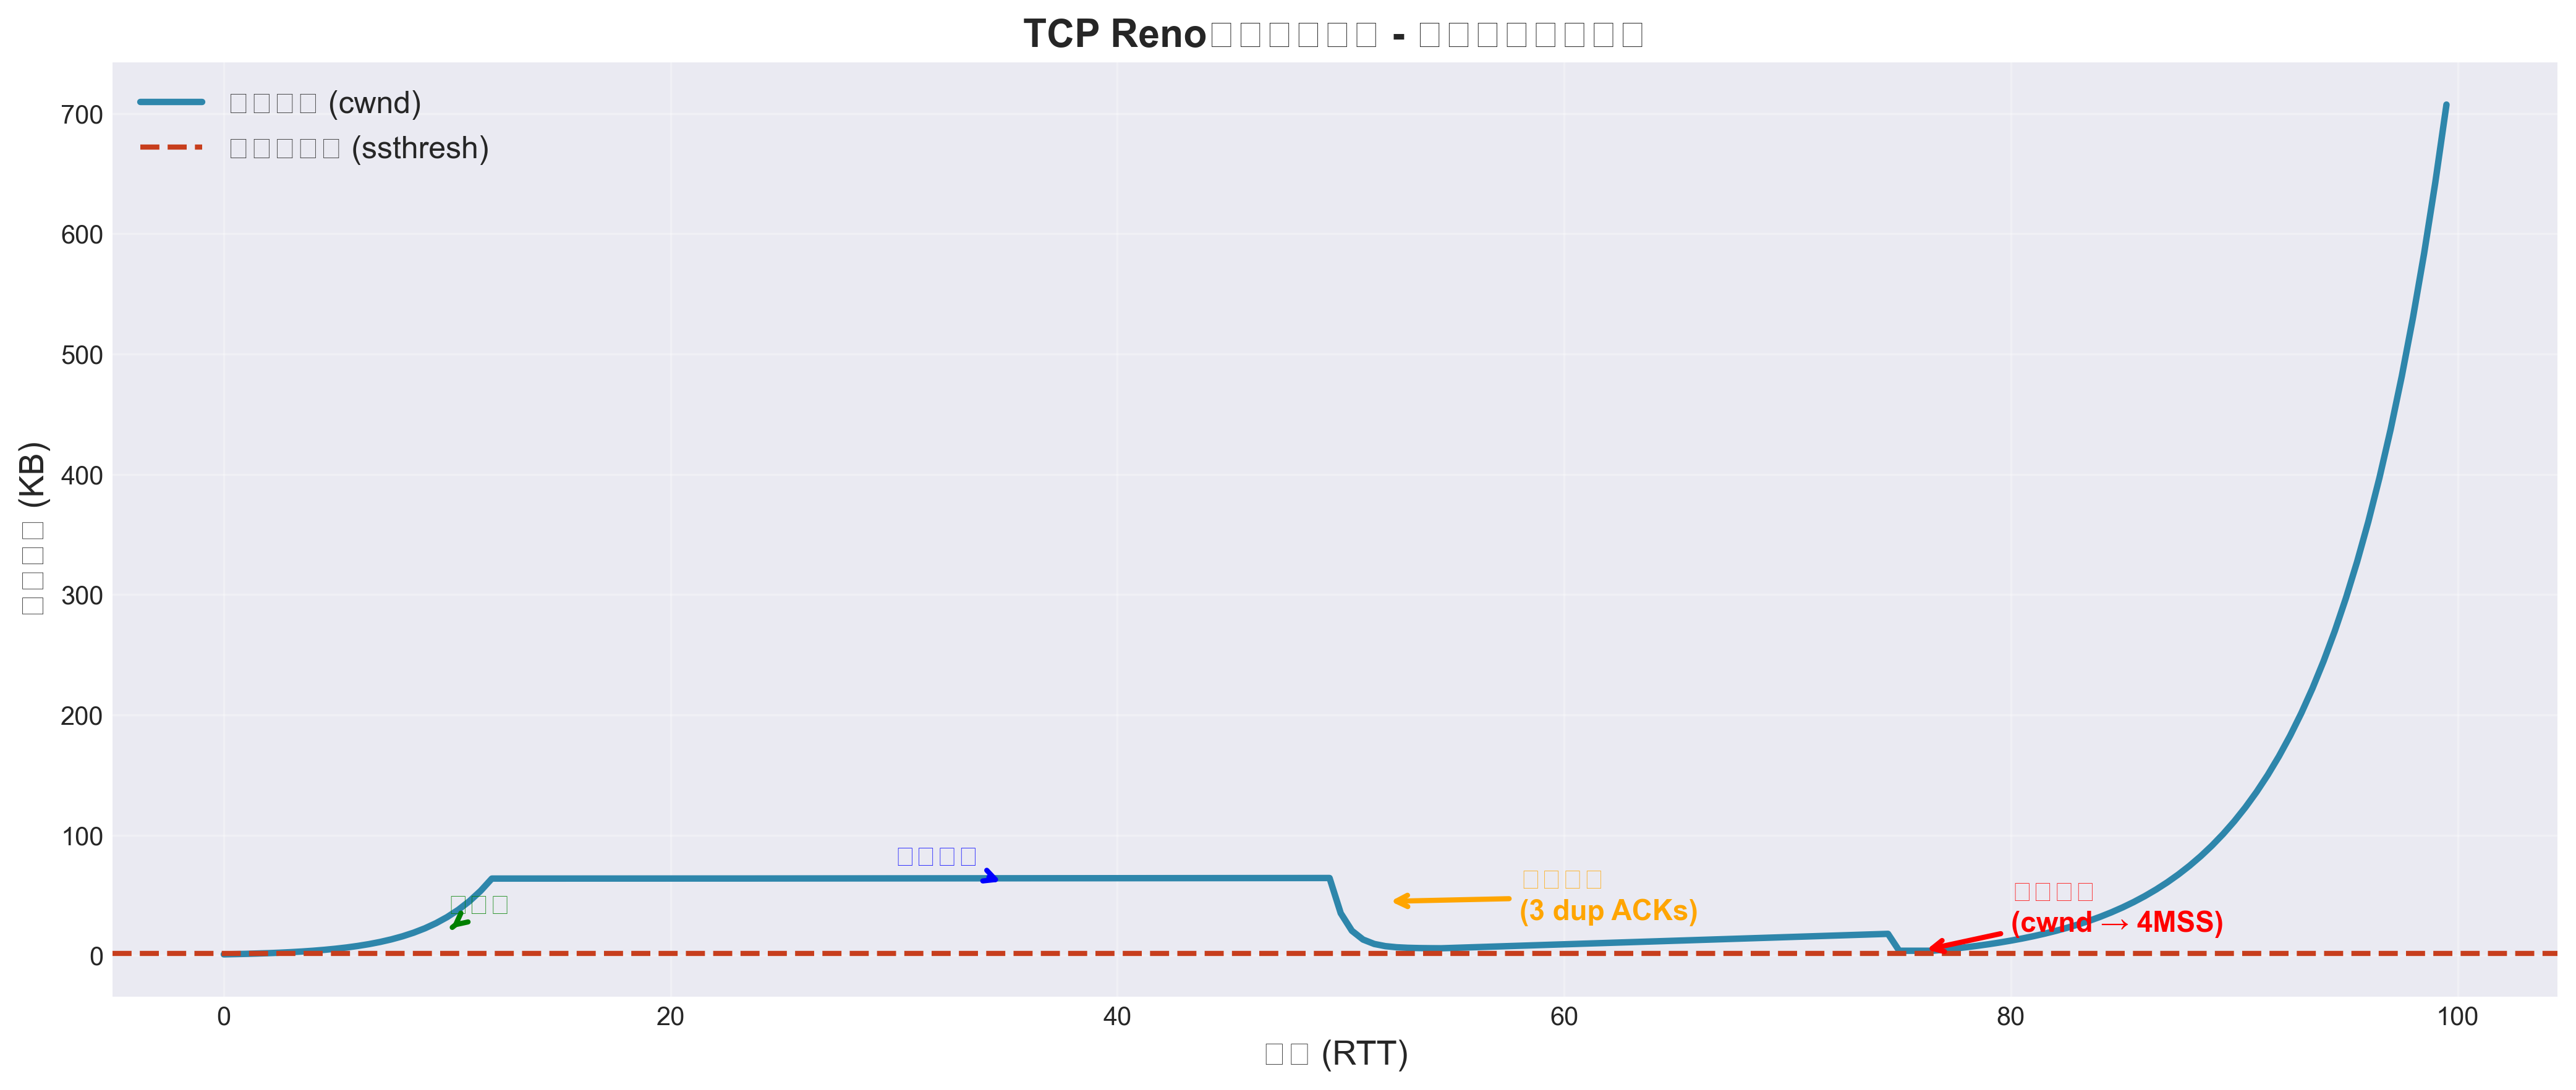
\includegraphics[width=0.95\linewidth]{cwnd_simulation.png}
    \caption{TCP Reno拥塞控制算法：拥塞窗口随时间的动态变化过程（模拟数据）}
    \label{fig:cwnd_sim}
\end{figure}

\subsection{多线程架构设计}
发送端采用高效的多线程模型，避免了阻塞IO带来的性能瓶颈：

\begin{itemize}
    \item \textbf{主线程}：负责读取文件、封装数据包、检查发送窗口可用性，并将数据推入网络。
    \item \textbf{监听线程 (Listener Thread)}：全时段监听Socket，接收ACK/SACK包。解析确认信息，更新 `base`、`cwnd`、`ssthresh` 等状态变量，并剔除发送缓冲区中已确认的包。
    \item \textbf{定时器线程 (Timer Thread)}：以10ms精度轮询 `send\_buffer`，检查头部数据包是否超时。一旦触发超时，执行重传并调整拥塞窗口（进入慢启动）。
\end{itemize}
线程间通过 `std::mutex` 对共享资源（如 `send\_buffer`、`cwnd`）进行保护，确保数据一致性。

\section{性能测试与分析}

\subsection{丢包率对性能的影响}
在延时固定为5ms，带宽限制不明显的条件下，测试了不同丢包率下的协议表现。

\begin{table}[H]
    \centering
    \caption{不同丢包率下的传输性能对比 (延时=5ms)}
    \label{tab:loss_impact}
    \begin{tabular}{c|c|c|c|c|c}
        \toprule
        \textbf{丢包率} & \textbf{传输时间(s)} & \textbf{吞吐率(Mbps)} & \textbf{重传包数} & \textbf{超时次数} & \textbf{重复ACK} \\
        \midrule
        0\%    & 37.79   & 0.393   & 10  & 10  & 10  \\
        0.5\%  & 54.37   & 0.273   & 19  & 10  & 139 \\
        1\%    & 53.90   & 0.276   & 19  & 1   & 264 \\
        2\%    & 54.92   & 0.271   & 38  & 1   & 378 \\
        3\%    & 77.19   & 0.193   & 58  & 2   & 424 \\
        \bottomrule
    \end{tabular}
\end{table}

\begin{figure}[H]
    \centering
    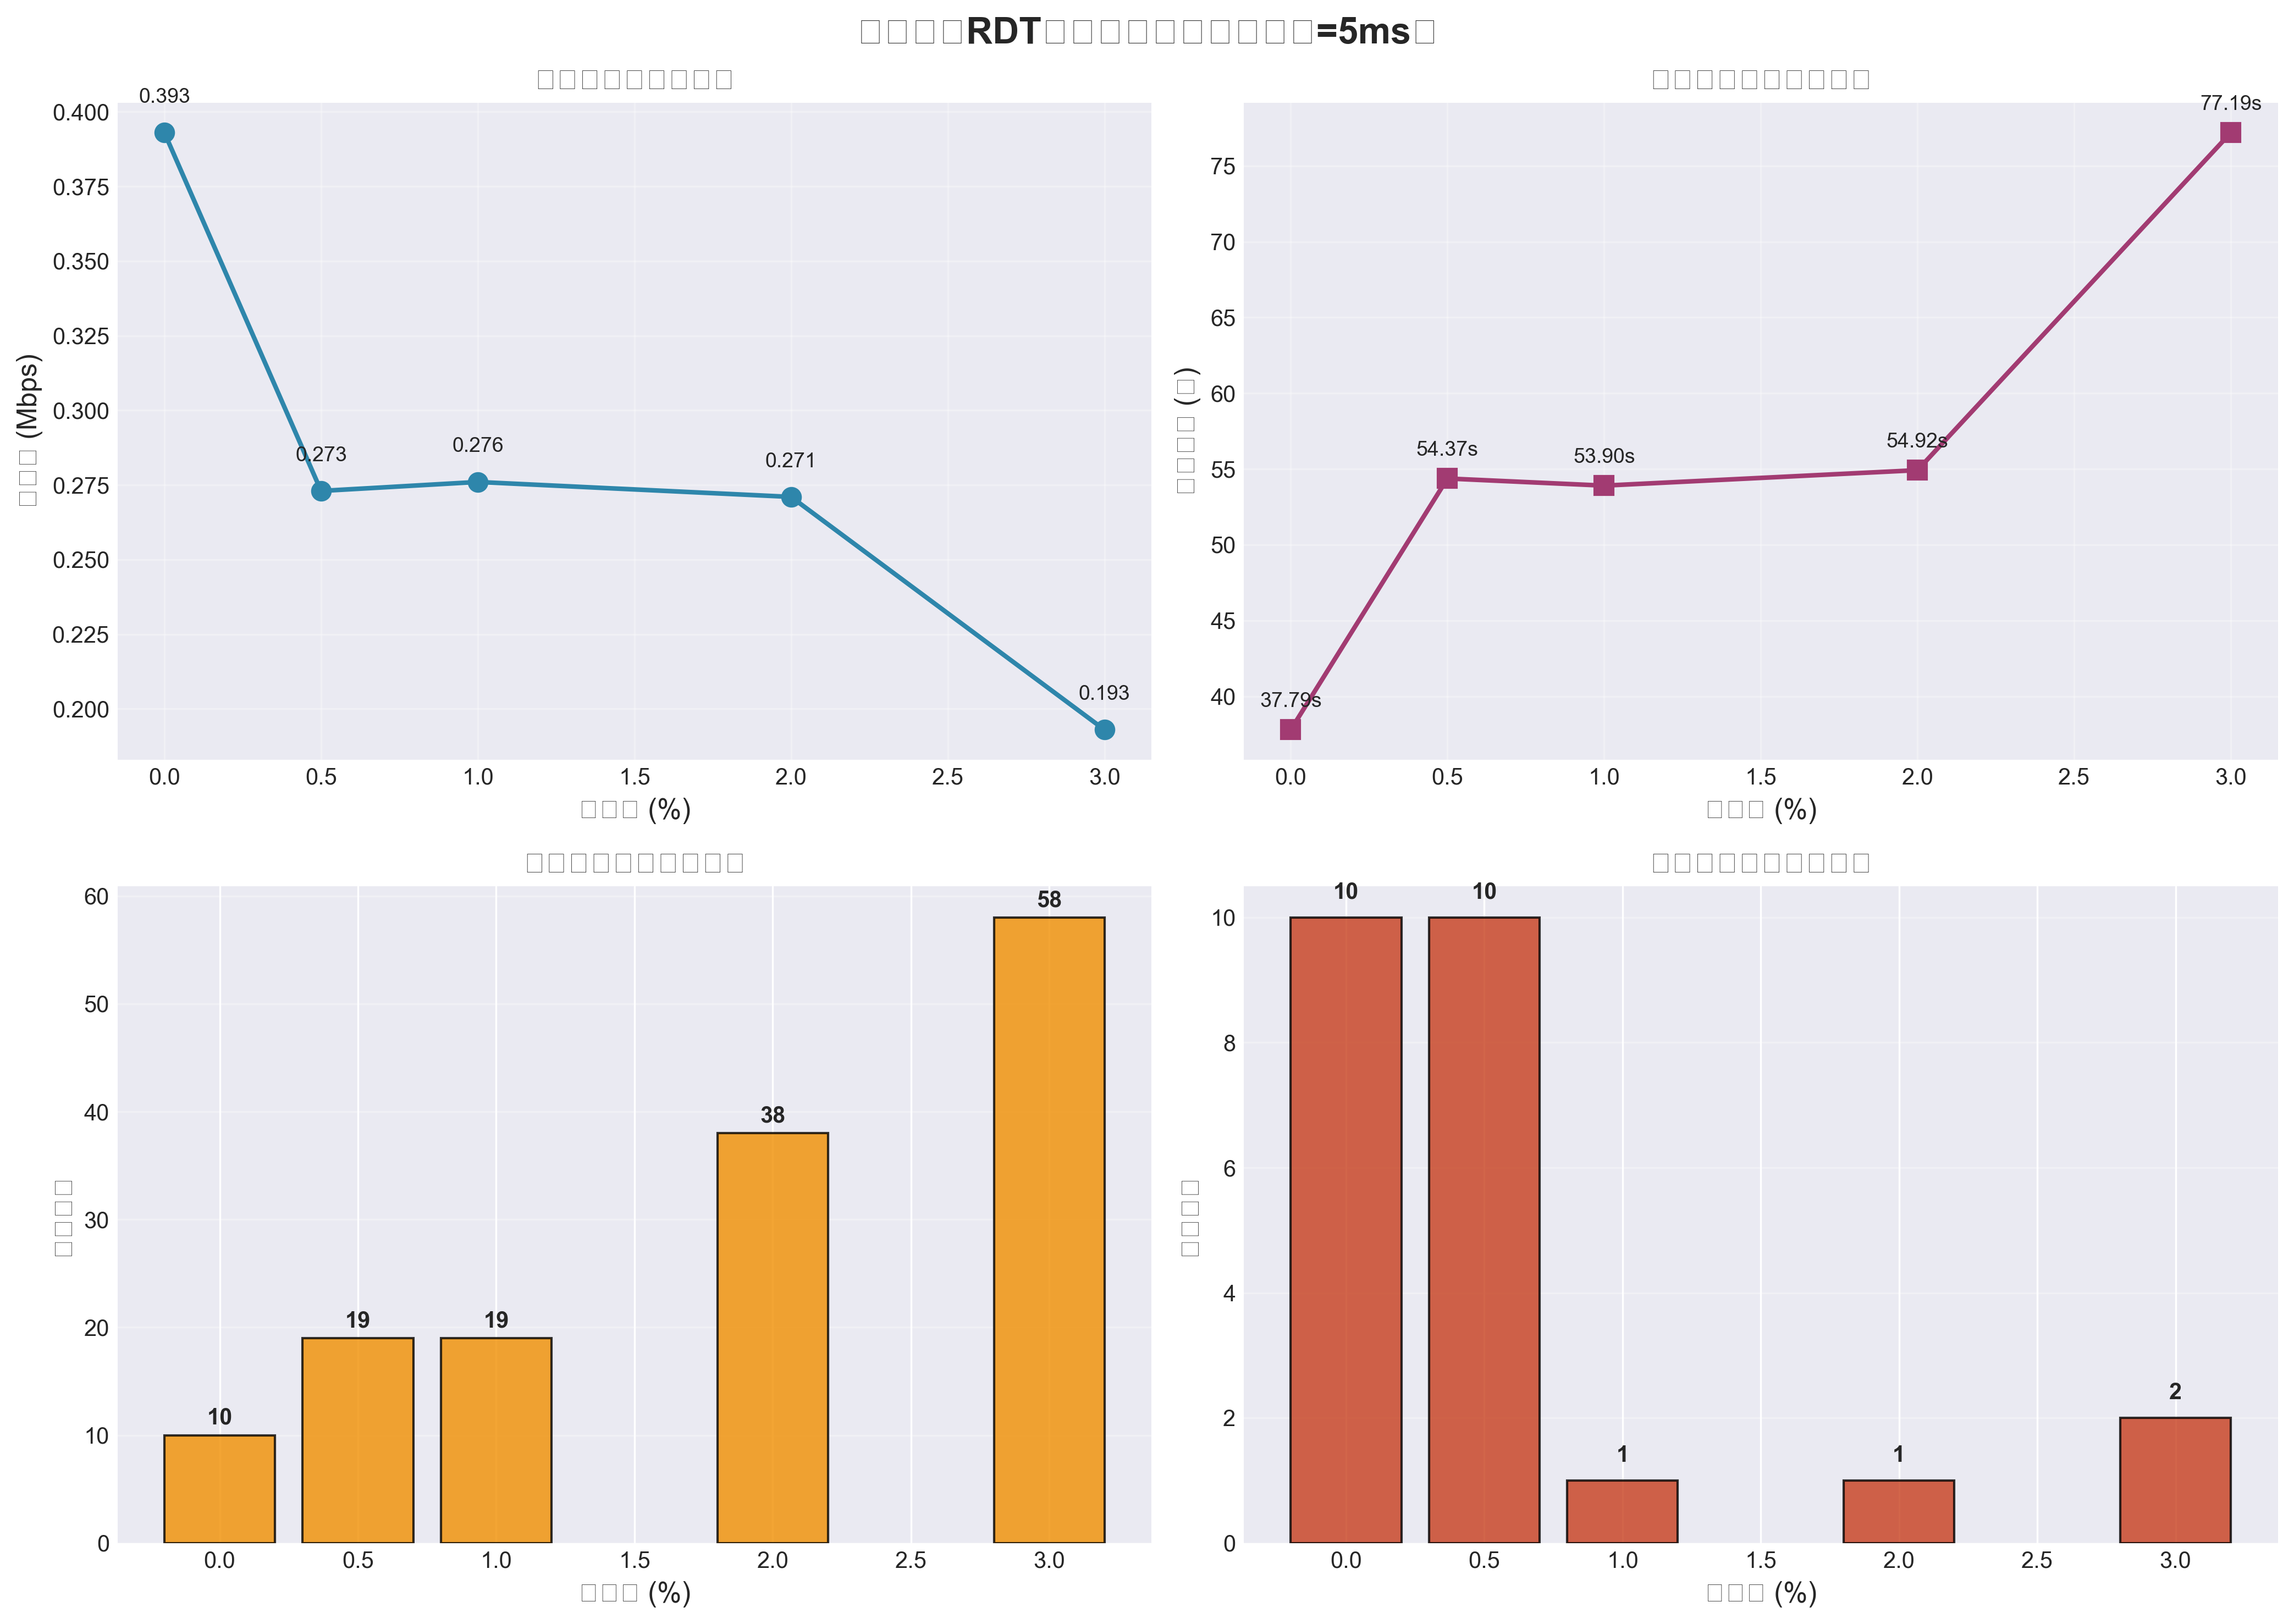
\includegraphics[width=0.9\linewidth]{loss_rate_impact.png}
    \caption{丢包率对吞吐率、传输时间及重传行为的影响分析}
    \label{fig:loss_charts}
\end{figure}

\textbf{分析}：
从表 \ref{tab:loss_impact} 和图 \ref{fig:loss_charts} 可以看出，随着丢包率的上升，吞吐率呈下降趋势。
\begin{enumerate}
    \item 在低丢包率（0.5\%-2\%）区间，吞吐率维持在0.27 Mbps左右，相对稳定。这说明**快速重传**和**SACK**机制发挥了显著作用，大部分丢包通过重复ACK触发重传修复，未触发昂贵的超时重传（超时次数仅为1次）。
    \item 当丢包率升至3\%时，传输时间显著增加（从54s增至77s），吞吐率跌至0.193 Mbps。重复ACK数量剧增（424次），表明网络拥塞加剧，发送端频繁进入快速恢复阶段，窗口无法持续增长，限制了吞吐率。
\end{enumerate}

\subsection{网络延时对性能的影响}
固定丢包率为0.1\%，测试不同链路延时（RTT $\approx$ 2 $\times$ Delay）下的性能。

\begin{table}[H]
    \centering
    \caption{不同延时下的传输性能对比 (丢包率=0.1\%)}
    \label{tab:delay_impact}
    \begin{tabular}{c|c|c|c|c}
        \toprule
        \textbf{单向延时} & \textbf{传输时间(s)} & \textbf{吞吐率(Mbps)} & \textbf{重传包数} & \textbf{超时次数} \\
        \midrule
        0ms     & 14.58   & 1.019   & 2    & 1   \\
        5ms     & 54.58   & 0.272   & 19   & 18  \\
        20ms    & 84.43   & 0.176   & 41   & 40  \\
        100ms   & 263.07  & 0.056   & 303  & 301 \\
        \bottomrule
    \end{tabular}
\end{table}

\begin{figure}[H]
    \centering
    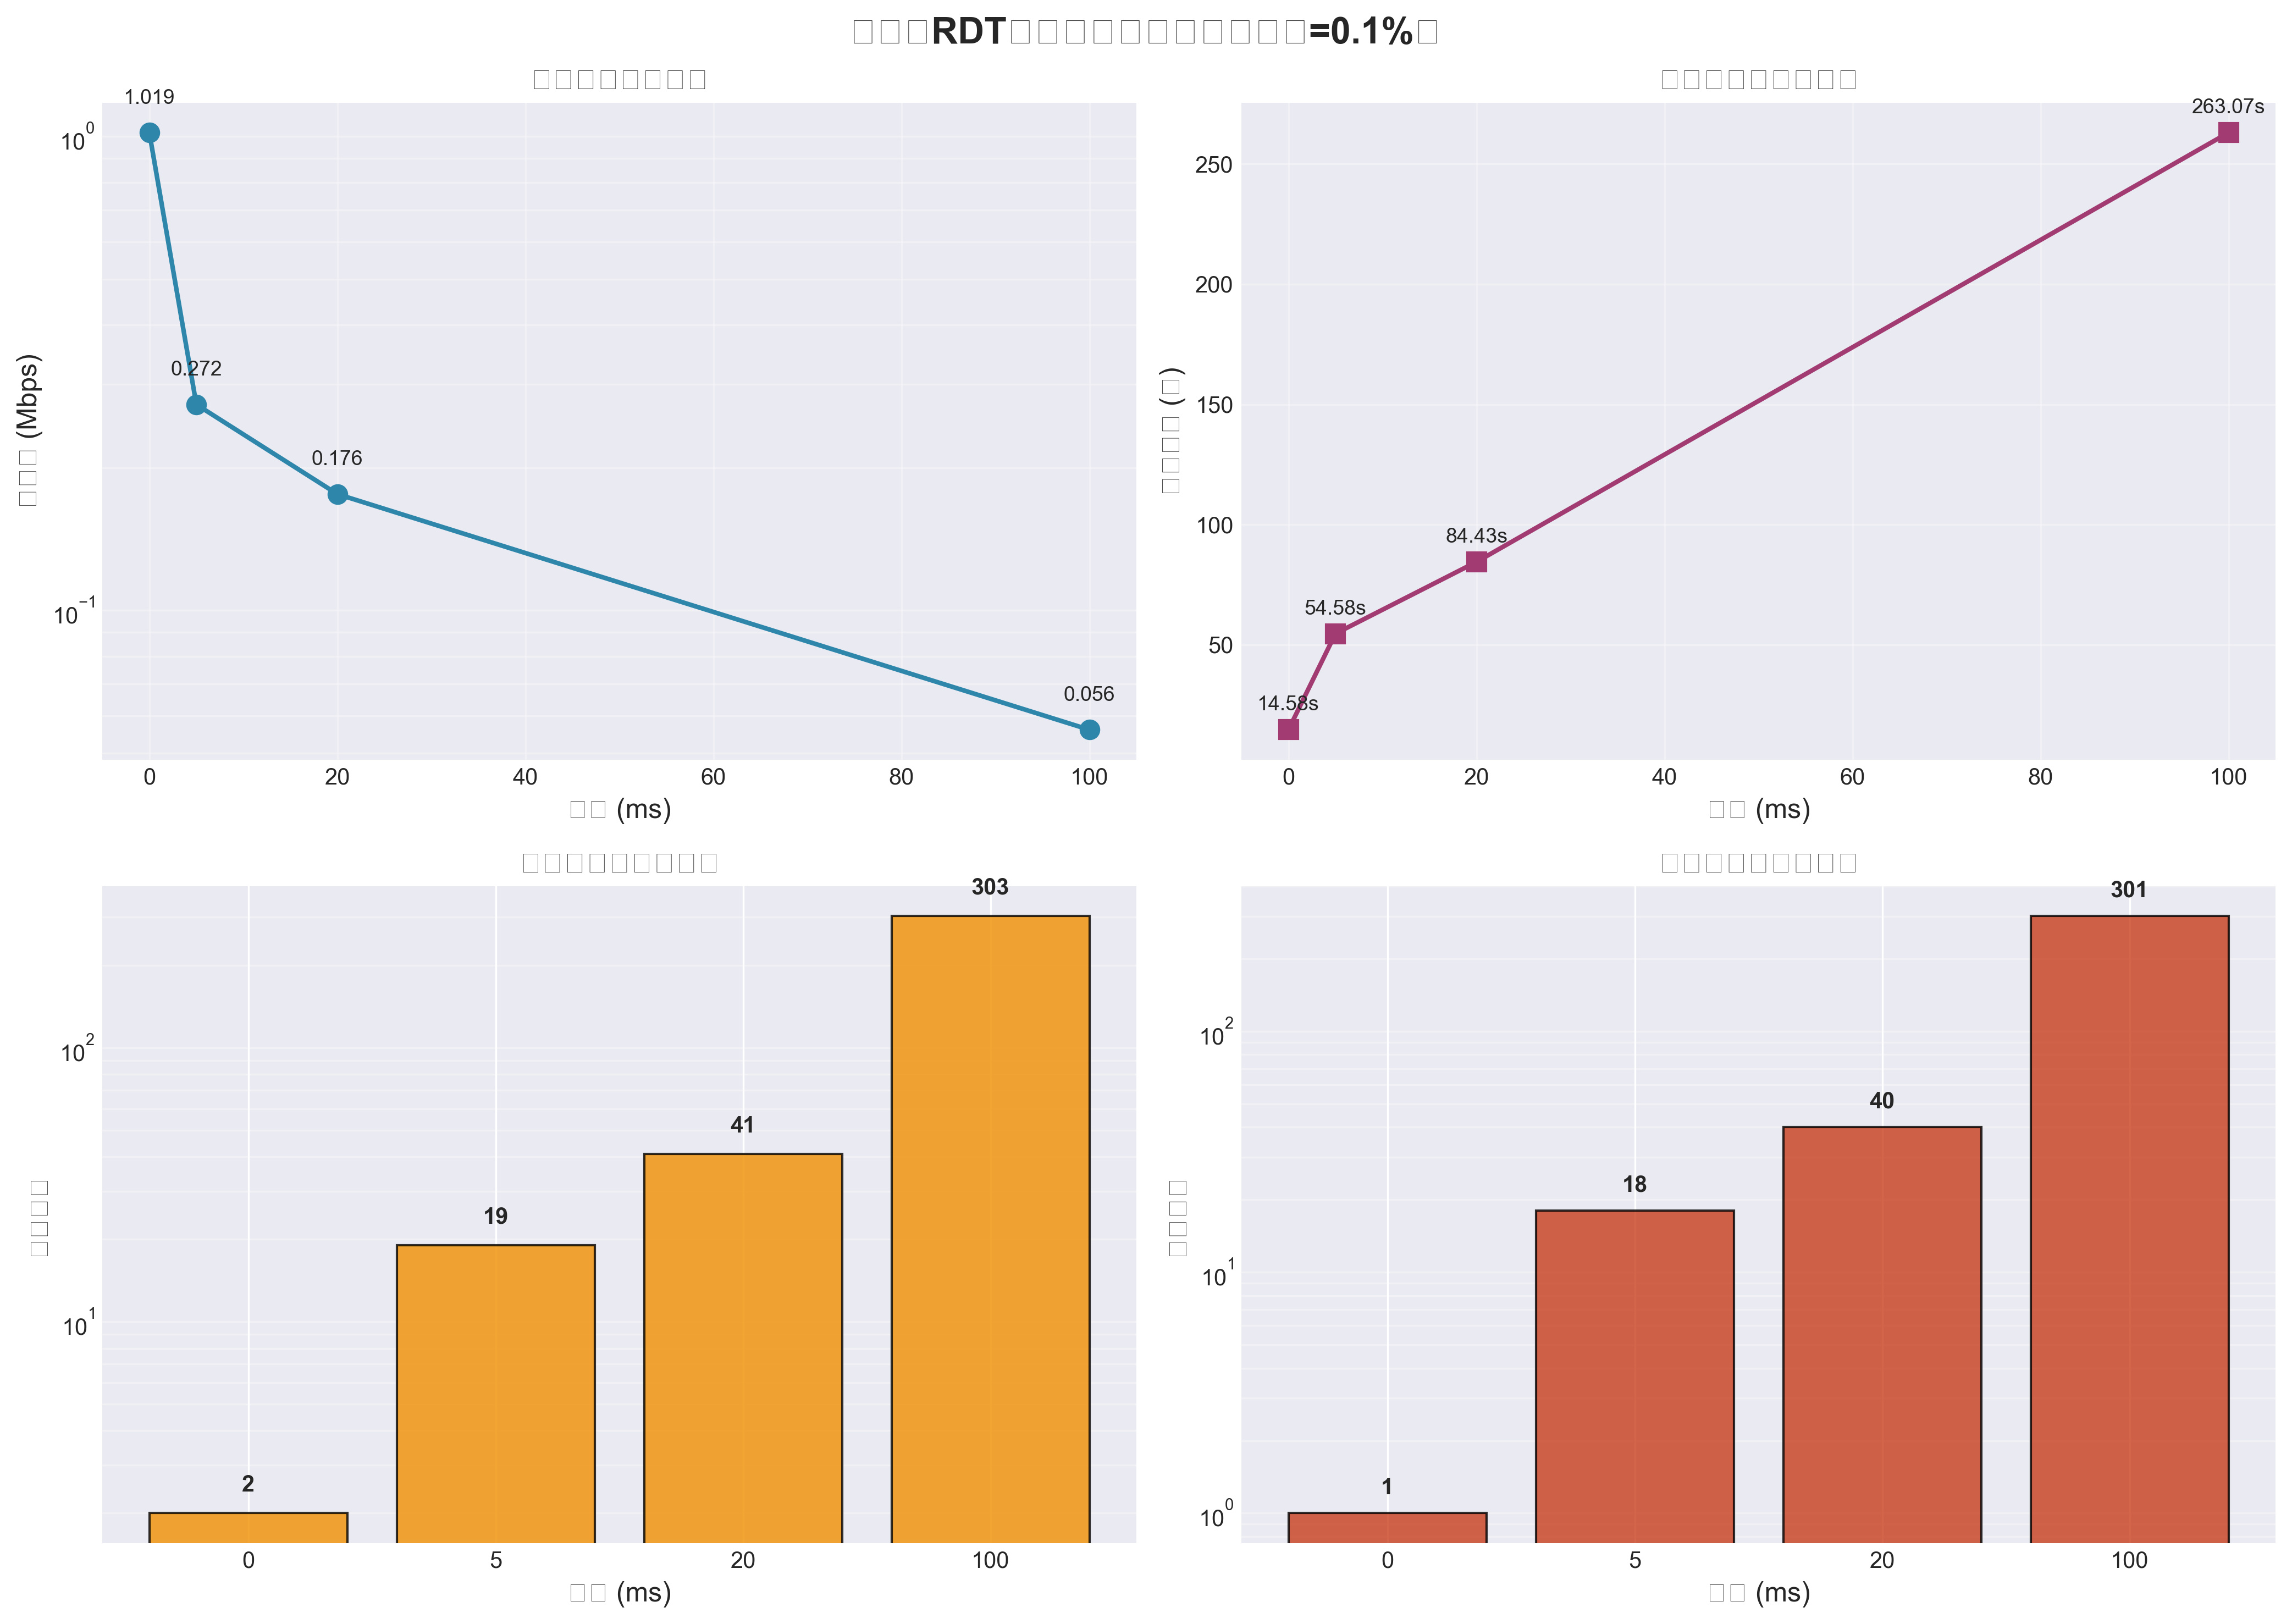
\includegraphics[width=0.9\linewidth]{delay_impact.png}
    \caption{延时对RDT协议各项性能指标的影响趋势}
    \label{fig:delay_charts}
\end{figure}

\textbf{分析}：
延时对性能的影响比丢包率更为剧烈（见图 \ref{fig:delay_charts}）。
\begin{itemize}
    \item \textbf{带宽时延积限制}：TCP吞吐率理论上限与 $\frac{1}{RTT}$ 成正比。随着延时增加，RTT增大，在窗口大小有限的情况下，信道利用率急剧下降。
    \item \textbf{超时激增}：在100ms高延时下，超时次数高达301次，几乎与重传包数持平。这表明固定的500ms超时设置在高RTT环境下可能过于激进，导致即使包未丢失，也因ACK返回过慢而触发虚假超时重传。这提示我们需要实现自适应的RTO（Retransmission Timeout）计算机制。
\end{itemize}

\subsection{理想与现实的差距}
最后，对比无路由器限制（理想环境）与有损环境的性能。

\begin{figure}[H]
    \centering
    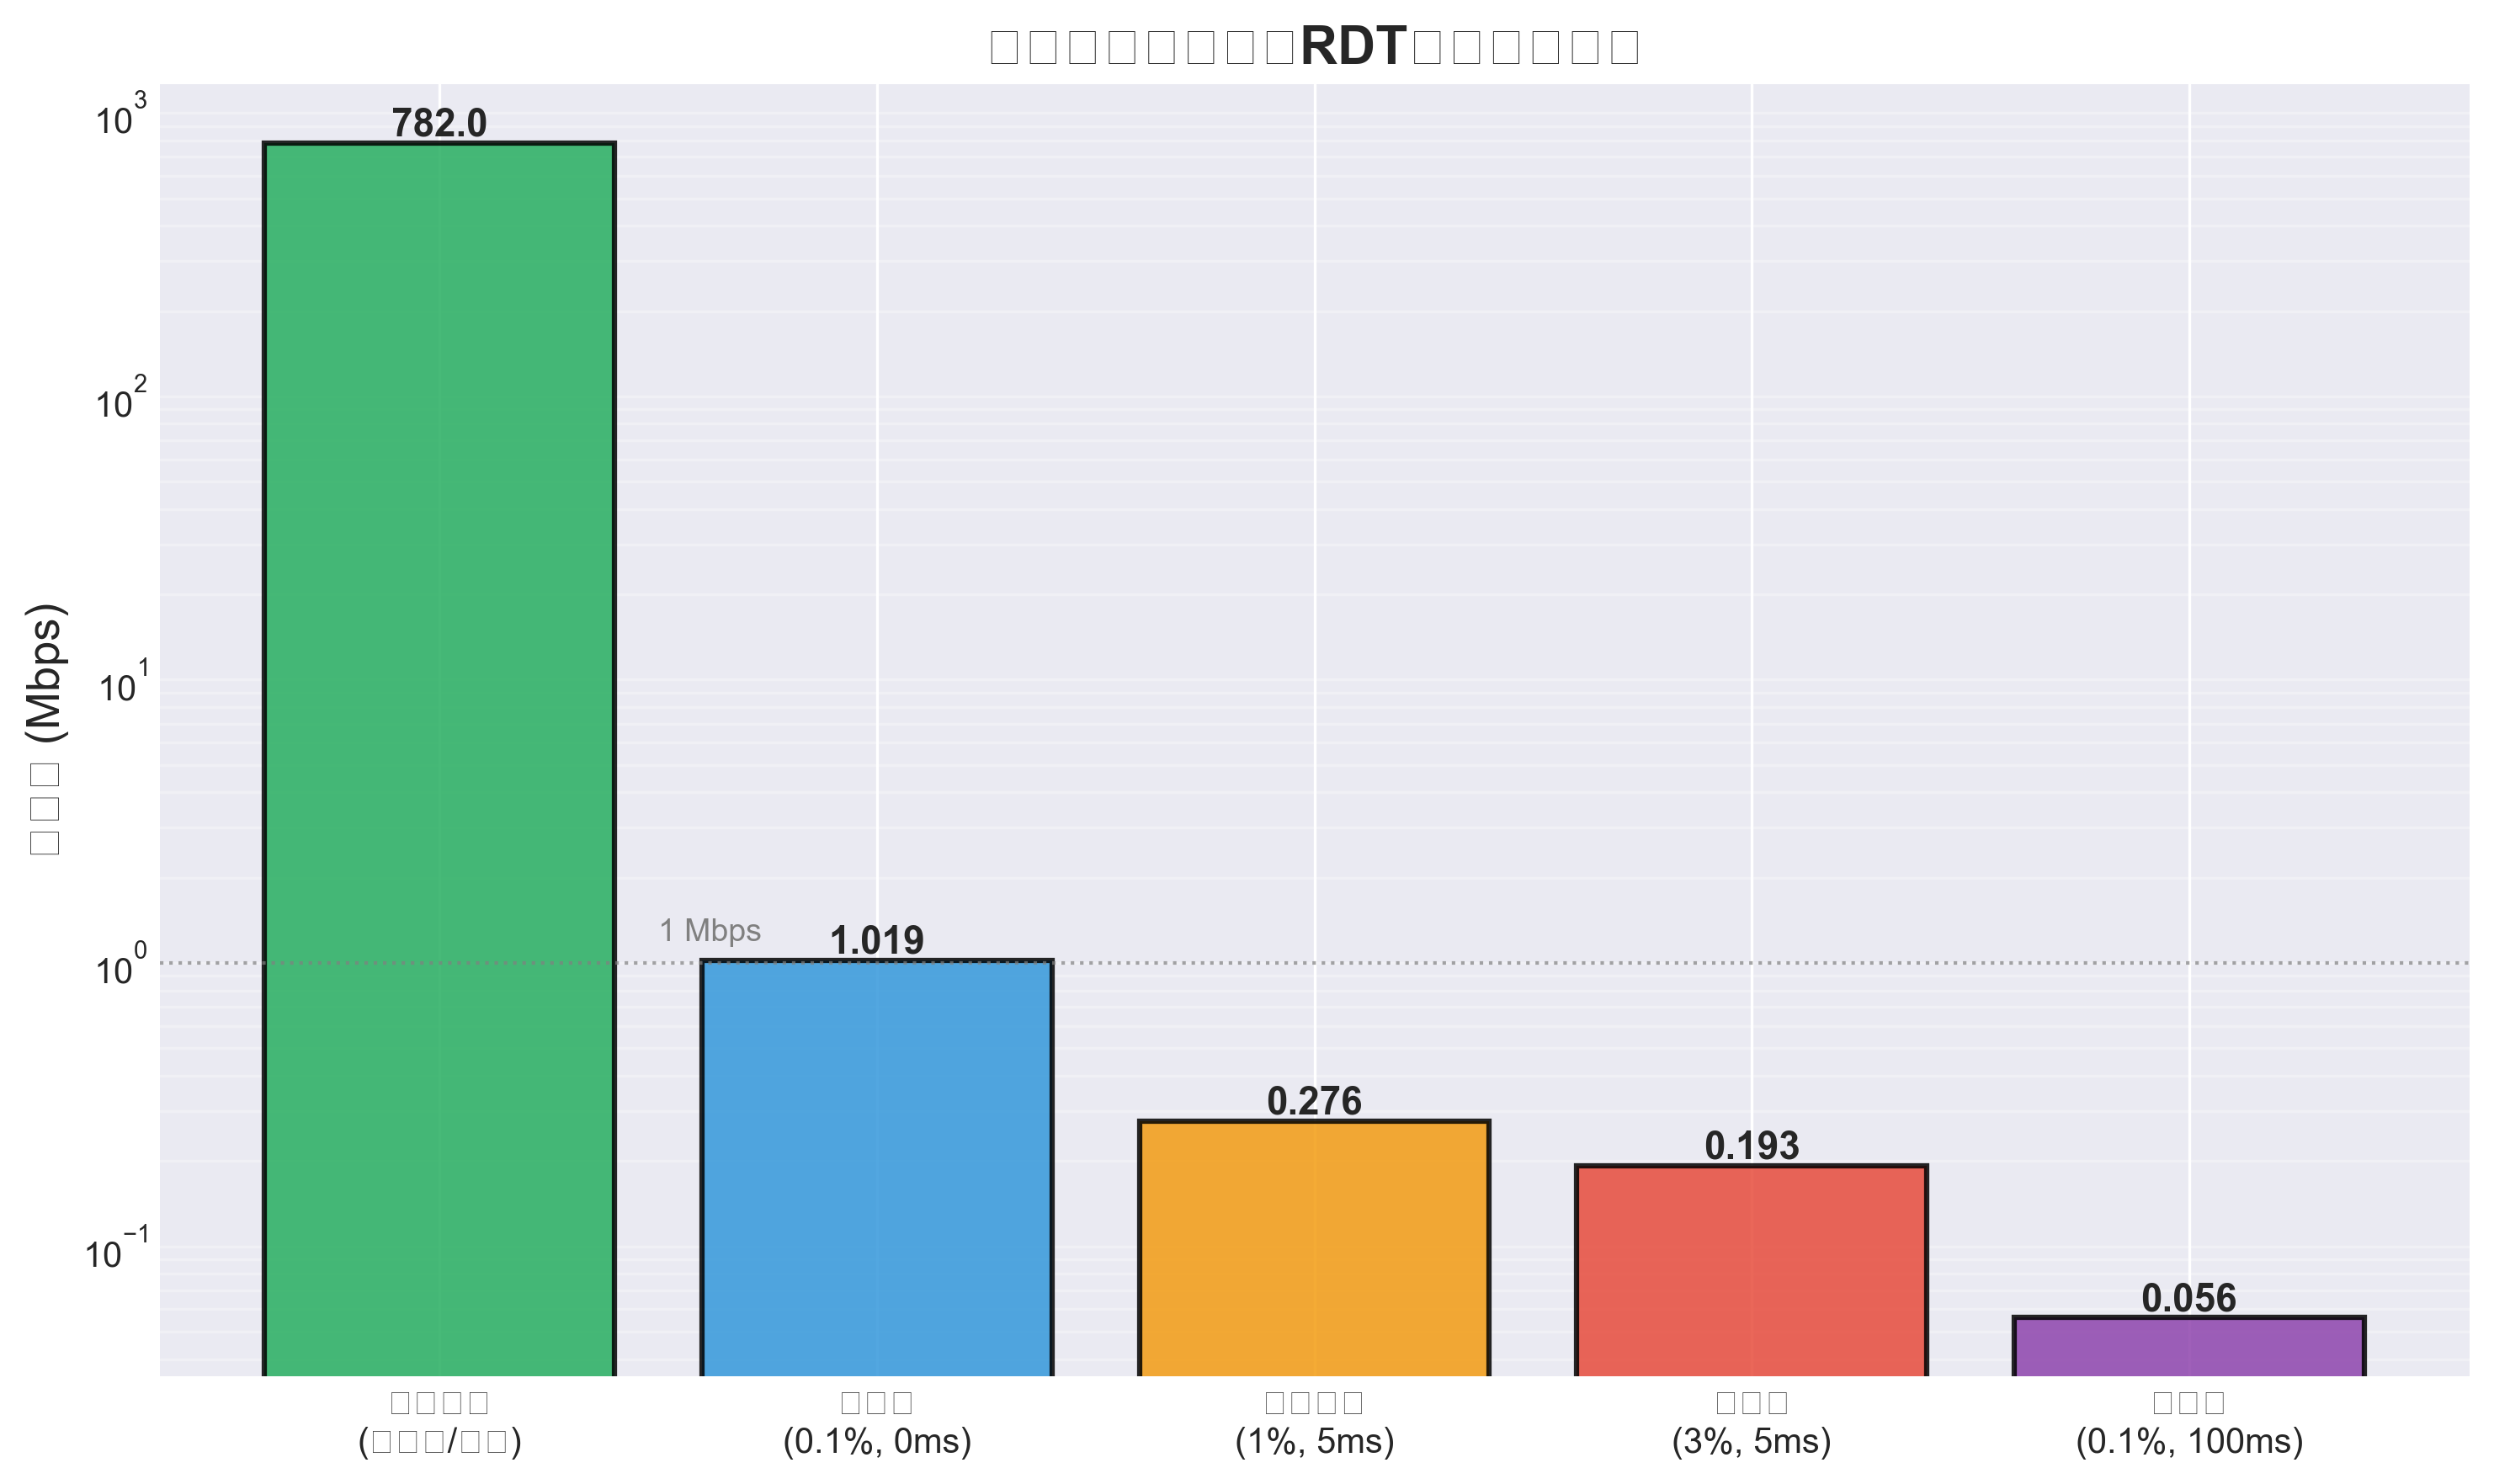
\includegraphics[width=0.8\linewidth]{performance_comparison.png}
    \caption{理想环境与各类有损网络环境下的吞吐率数量级对比}
    \label{fig:perf_compare}
\end{figure}

如图 \ref{fig:perf_compare} 所示，在本地环回且无模拟损耗时，协议吞吐率高达782 Mbps（1.jpg测试数据），受限于CPU处理速度和IO性能。引入极小的损耗（0.1\%, 0ms）后，吞吐率骤降至1 Mbps级别。这凸显了拥塞控制算法为了保障可靠性，不得不在发送速率上做出巨大牺牲。

\section{总结}

\subsection{实验成果}
本实验成功实现了一个功能完备的RDT协议。代码结构清晰，通过 `sender.cpp` 和 `receiver.cpp` 的协同工作，实现了：
\begin{enumerate}
    \item \textbf{健壮的连接管理}：能够正确处理握手和挥手，即使在丢包环境下也能最终完成状态同步。
    \item \textbf{高效的丢包恢复}：结合SACK和NewReno算法，有效应对了连续丢包场景，避免了吞吐率的断崖式下跌。
    \item \textbf{精确的拥塞控制}：通过日志观察，确认拥塞窗口 `cwnd` 能够根据网络反馈动态调整，符合Reno算法的行为特征。
\end{enumerate}

\subsection{关键发现与改进方向}
通过对测试数据的深入分析，我发现：
\begin{itemize}
    \item \textbf{固定RTO的局限性}：在100ms延时测试中性能极差，说明硬编码的500ms超时时间缺乏适应性。未来应实现Jacobson/Karels算法，根据测量到的RTT动态计算RTO。
    \item \textbf{Partial ACK的重要性}：在NewReno实现中，正确识别Partial ACK并立即重传后续丢失包，是防止协议在快速恢复阶段"卡死"或退回到慢启动的关键。
    \item \textbf{发送窗口优化}：当前的发送策略较为激进，未实现Nagle算法，对于小数据包传输效率较低，未来可予以改进。
\end{itemize}

本次实验不仅锻炼了我的编码能力，更让我对TCP协议中那些精妙的设计思想——如"慢启动"的审慎、"快速重传"的果断——有了直观而深刻的感悟。

\end{document}
